\documentclass[11pt]{article}
\usepackage[utf8]{inputenc}	% Para caracteres en español
\usepackage{amsmath,amsthm,amsfonts,amssymb,amscd}
\usepackage{multirow,booktabs}
\usepackage[table]{xcolor}
\usepackage{fullpage}
\usepackage{lastpage}
\usepackage{enumitem}
\usepackage{fancyhdr}
\usepackage{mathrsfs}
\usepackage{wrapfig}
\usepackage{setspace}
\usepackage{calc}
\usepackage{multicol}
\usepackage{cancel}
\usepackage[retainorgcmds]{IEEEtrantools}
\usepackage[margin=3cm]{geometry}
\usepackage{amsmath}
\newlength{\tabcont}
\setlength{\parindent}{0.0in}
\setlength{\parskip}{0.05in}
\usepackage{empheq}
\usepackage{framed}
\usepackage[most]{tcolorbox}
\usepackage{xcolor}
\colorlet{shadecolor}{orange!15}
\parindent 0in
\parskip 12pt
\geometry{margin=1in, headsep=0.25in}
\theoremstyle{definition}
\newtheorem{defn}{Definition}
\newtheorem{reg}{Rule}
\newtheorem{exer}{Exercise}
\newtheorem{note}{Note}
\usepackage{listings}
\usepackage{xcolor}
\usepackage{graphicx}
\graphicspath{ {./images/} }
\newcommand*{\Co}[2]{{}^{#1}C_{#2}}%
\lstset { %
    language=C++,
    backgroundcolor=\color{black!5}, % set backgroundcolor
    basicstyle=\footnotesize,% basic font setting
}
\begin{document}
\title{Week 1 Notes}
\thispagestyle{empty}

\begin{center}
{\vspace{5mm} \LARGE ECE 250 - Fall 2018 \\ \vspace{5mm}Aditya Arora}\\
{\vspace{5mm} \LARGE \bf Week 1 Notes}

\end{center}
\section{Introduction}

\textbf{Key details given on Course Outline, Project submissions and Policy 71}

\section{Mathematical background}
\subsection{Floor and Ceiling Functions}
Floor: The \textit{floor} function maps any real number \textit{x} onto the greatest integer less than or equal to \textit{x} 
\newline
- Consider it to be rounding towards \textit{negative infinity}
Example: floor(0.5) == 0, floor(3.2) == 3

Ceiling: The \textit{ceilling} function maps any real number \textit{x} onto the least integer integer greater than or equal to \textit{x} 
\newline
- Consider it to be rounding towards \textit{positive infinity}
Example: ceil(0.5) == 1, ceil(3.2) == 4
\newline
\begin{lstlisting}
// Both of these functions are implemented in the cmath library
# include <cmath>

double floor(double);
double ceil(double);

/*
They're doible because double has a greater range (just under 2^1024) 
over long which can represent upto (2^63-1)
*/
\end{lstlisting}

\subsection{L’Hôpital’s rule}
If you are trying to determine: $\mathop {\lim }\limits_{x \to c} \frac{{f\left( x \right)}}{{g\left( x \right)}}$
but both $\mathop {\lim }\limits_{x \to c}{f\left( x \right)} = \infty$ and $\mathop {\lim }\limits_{x \to c}{g\left( x \right)} = \infty$
$$\mathop {\lim }\limits_{x \to c} \frac{{f\left( x \right)}}{{g\left( x \right)}} = \mathop {\lim }\limits_{x \to c} \frac{{f'\left( x \right)}}{{g'\left( x \right)}}$$
This rule can be repeated as necessary

\newpage

\subsection{Logarithms and Exponentials}
\begin{itemize}[label={--}]
\item If  $n = e^m$, we define
$m = ln(n)$. It is always true that $e^{ln(n)} = n$; however, $ln(e^n)$ = n requires that n is real 
\item Exponentials grow faster than any non-constant polynomial
$$\mathop {\lim }\limits_{n \to \infty}\frac{e^n}{n^d} = \infty$$ for any $d > 0$
\item Logarithms grow slower than any polynomial
$$\mathop {\lim }\limits_{n \to \infty}\frac{ln(n)}{n^d} = 0$$ for any $d > 0$
\item All logarithms are linear multiples of each other
$$log_{b}(n) = \frac{ln(n)}{ln(b)}$$
\item \begin{lstlisting}
// the base-2 logarithm log2(n) is written as lg(n)

double log(double); //ln(n)
double log10(double); //log10(n)
\end{lstlisting}
\item $m^{log_{b}(n)} = n^{log_{b}(m)}$
\end{itemize}
\newpage
\subsection{Series}
\subsubsection{Arithmetic Series}
Each term in an arithmetic series is increased by a constant value (usually 1):
$$0 + 1 + \ldots + n = \sum_{k=0}^{n} k = \frac{n(n+1)}{2}$$
$$0^2 + 1^2 + \ldots + n^2 = \sum_{k=0}^{n} k^2 = \frac{n(n+1)(2n+1)}{6}$$
$$0^3 + 1^3 + \ldots + n^3 = \sum_{k=0}^{n} k^3 = (\frac{n(n+1)}{4})^2$$
To generalise: $$\sum_{k=0}^{n} k^d \approx \int_{0}^{n} x^d dx = \frac{n^{d+1}}{d+1}$$
The relative error of approximation of the equation goes to zero as $n$ tends to $\infty$

\subsubsection{Geometric Series}
The next series we will look at is the geometric series with common ratio r:
$$\sum_{k=0}^{n} r^k = \frac{1-r^{n+1}}{1-r}$$
and if $|r| < 1$ then it is also true that
$$\sum_{k=0}^{\infty} r^k = \frac{1}{1-r}$$

\newpage
\subsection{Recurrence Relations}
\begin{itemize}[label={--}]
\item A recurrence relationship is a means of defining a sequence based on previous values in the sequence.
\item Such definitions of sequences are said to be \textit{recursive}
\item
\begin{shaded}
Define an initial value: e.g., $x_1 = 1$
\newline
Defining $x_n$ in terms of previous values:
For example,
	  		$$x_n = x_{n – 1} + 2$$
			$$x_n = 2x_{n – 1} + n$$
			$$x_n = x_{n – 1} + x_{n – 2}$$
\end{shaded}
\end{itemize}
\subsection{Weighted Average}
Given n objects $x_1, x_2, x_3, \ldots, x_n$, the average is
$$\frac{x_1+x_2+x_3\ldots+x_n}{n}$$
	Given a sequence of coefficients $c_1 , c_2 , c_3 ,\ldots, c_n$ where
$$c_1 + c_2 + \ldots + c_n = 1$$
then we refer to:
$$\frac{c_1x_1+c_2x_2+c_3x_3\ldots+c_nx_n}{n}$$	as a weighted average \newline
For an average, $c_1 = c_2 = \ldots = c_n = 1$
\newline
Examples:
\newline
\begin{minipage}{0.4\textwidth}
\begin{itemize}[label={--}]
\item Simpson’s method approximates an integral by sampling the function at three points:  f(a), f(b), f(c)
\item The average value of the function is approximated by
\end{itemize}
\end{minipage}%
%
\begin{minipage}{0.4\textwidth}
\begin{center}
    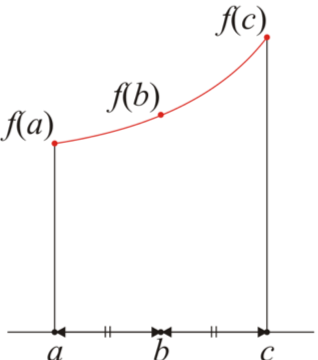
\includegraphics[width=0.6\textwidth]{simmons}
    \label{img:g}
\end{center}
\end{minipage}

\subsection{Combinations}
Given n distinct items, in how many ways can you choose k of these?
The number of ways such items can be chosen is written:
$$\Co{n}{k} = \frac{n!}{(k!)(n-k)!}$$

This is also a recursive definition:
$\Co{n}{k} = \Co{n-1}{k} + \Co{n-1}{k-1}$

\begin{itemize}[label={--}]
\item These are also the co-efficients of Pascal's Triangle
\item They are also the coefficients that we use to expand $(x+y)^n$
\end{itemize}



\end{document}